\section{Lezione 2016-10-21}
\subsection{TODO}
% Insert what you need. Any row is associated with the improvment or mistake
% arise. In the first column you can insert what you should resolve or change,
% instead in the second column you may put the section where to apply some
% modification.
\begin{table}[H]
\begin{center}
\begin{tabular}{|p{\textwidth}|c|}
\hline
\multicolumn{1}{|c|}{\textbf{Miglioramento}} & \textbf{Sezione} \\ \hline
Capire perch\'e \`e difficile riordinare il codice &
\ref{sec:triples} \\ \hline
\end{tabular}
\end{center}
\caption{Tabella miglioramenti}
\label{tab:tab_todo}
\end{table}

\subsection{Generatore codice intermedio}
Lo scopo del codice intermedio \`e \textbf{facilitare il retargeting}:
riutilizzare i \textit{front-end} esistenti modificando, o creando, un
\textit{back-end} compatibile con la nuova macchina obiettivo. Ovviamente segue
la l'idea di il riutilizzo del codice inserendo uno stato d'astrazione
superiore, ovvero il codice intermedio.

\begin{figure}[H]
  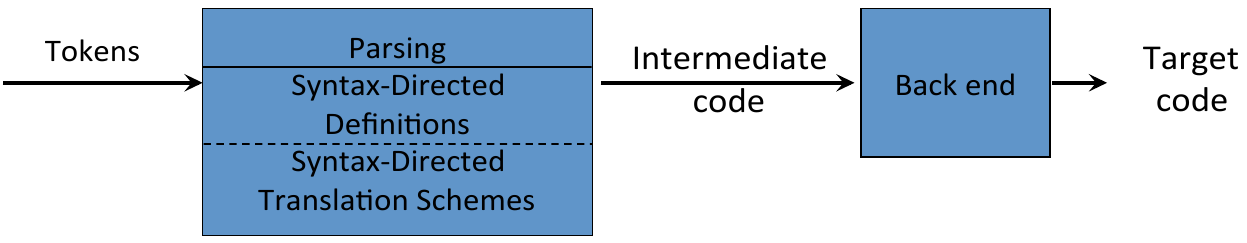
\includegraphics[scale=0.4]{res/image/compiler_backend}
  \caption{Codice intermedio, ponte tra \textit{front-end} e \textit{back-end}}
  \label{img:compiler_backend}
\end{figure}

\`E da specificare che il "codice" intermedio \`e pi\`u la rappresentazione
di come il \textit{front-end} comunica le azioni semantiche al
\textit{back-end} specificate nel sorgente del programma. Possibili
rappresentazioni sono:
\begin{itemize}
\item Rappresentazioni grafiche (es. AST e DAG)
\item Notazioni postfissa (simile alla JVM)
\item \textbf{Three-address code}: $x := y \ op \ z$
\item Two-address code ($x := op \ y$)
\end{itemize}

\subsubsection{Rappresentazioni grafiche - AST}
Utilizzando la \textit{Syntax-Directed Translation Table} si va a definire,
nelle \textit{semantic rules}, la costruzione dell'AST.

\begin{figure}[H]
  \centering
  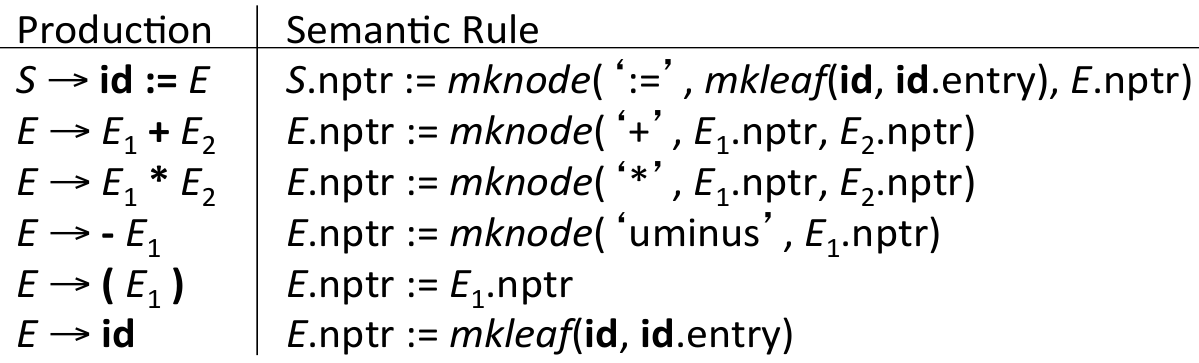
\includegraphics[scale=0.4]{res/image/ast_rappresentation}
  \caption{Codice intermedio con un AST}
  \label{img:ast_rappresentation}
\end{figure}

\paragraph{pro}
Facile ristrutturare il codice e/o espressione per ottimizzare il codice
intermedio.
\paragraph{cons}
Uso abbondante di memoria.

\subsubsection{Rappresentazioni grafiche - DAG}
Una via per sopperire il consumo di memoria nell'utilizzo di un AST \`e la
condivisione dei sottoalberi comuni tra pi\`u nodi genitori. La differenza tra
DAG e AST \`e nell'implementazione della costruzione dell'albero, dove i
metodi \textit{mkleaf} e \textit{mknode} \textbf{non creano} un nuovo nodo se
questo \`e gi\'a esistente.

\begin{figure}[H]
  \centering
  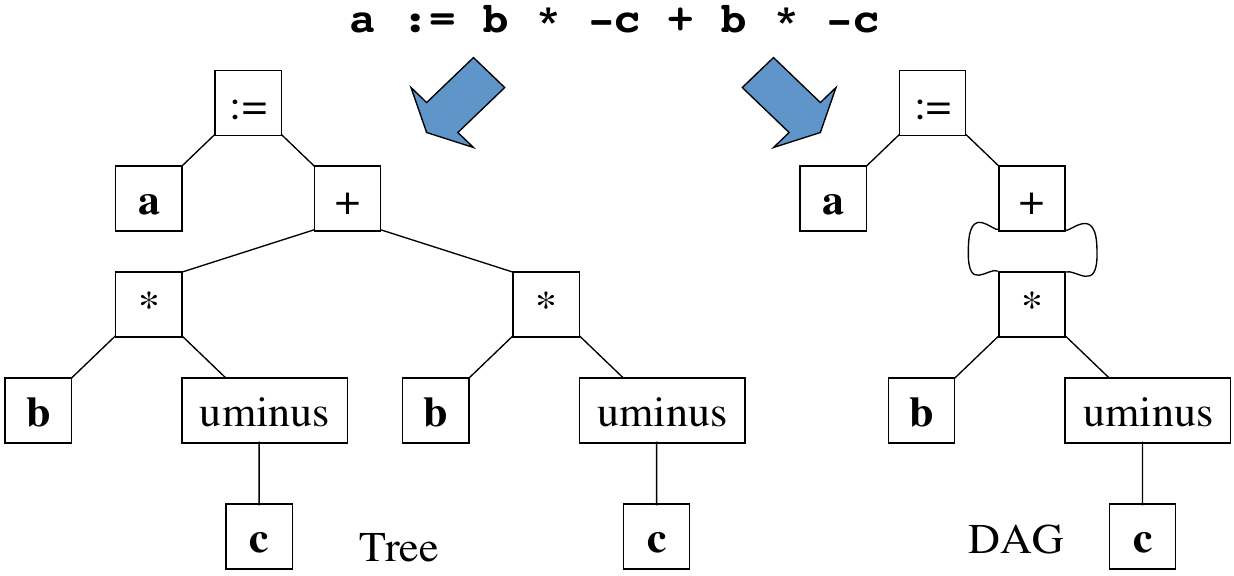
\includegraphics[scale=0.4]{res/image/dag_rappresentation}
  \caption{Codice intermedio con un DAG}
  \label{img:dag_rappresentation}
\end{figure}

\subsubsection{Notazione postfissa}
Tramite le \textit{semantics rules} abbiamo visto come disporre i termini delle
espressioni ponendo gli operandi sempre a sinistra e lo operazioni in fondo a
destra. L'ordinamento proposto va a rappresentare le \textbf{operazioni nello
stack} in cui dopo \`e immediato convertirlo nel codice intermedio
(es. bytecode).

\begin{figure}[H]
  \centering
  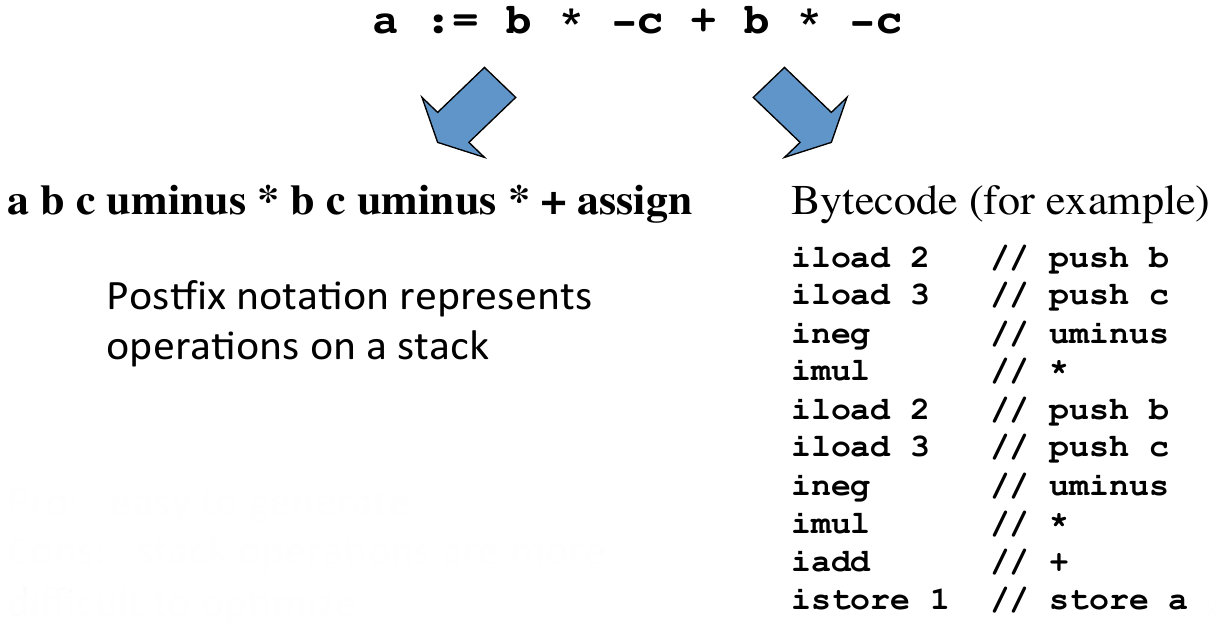
\includegraphics[scale=0.3]{res/image/postfix_rappresentation}
  \caption{Codice intermedio con notazione postfissa}
  \label{img:postfix_rappresentation}
\end{figure}

\paragraph{pro}
Semplice da generare.
\paragraph{cons}
Operazioni nello stack sono molto difficile da ottimizzare.

\subsubsection{Three-Address Code}
Dato l'AST dell'espressione il \textit{Three-Address Code} \`e ottenuto
mediante l'attraversamento \textit{depth-first} dell'albero, costruendone una
sua rappresentazione lineare.

\begin{figure}[H]
  \centering
  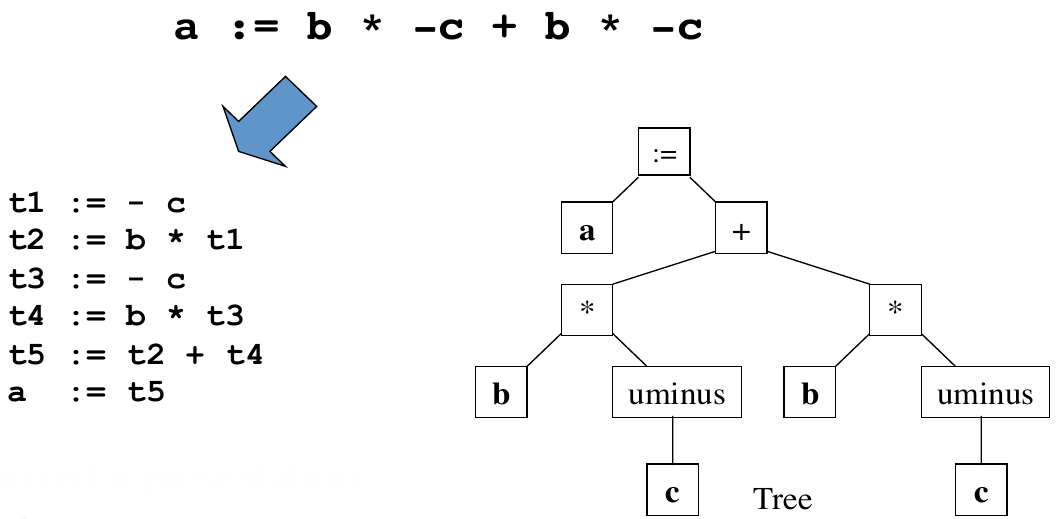
\includegraphics[scale=0.35]{res/image/tac_rappresentation}
  \caption{Codice intermedio con \textit{Three-Address Code}}
  \label{img:tag_rappresentation}
\end{figure}

Per un risparmio sulla memoria impiegata per la costruzione dell'AST si va a
ricorrere all'uso del DAG. La metodologia di conversione nel
\textit{three-address code} ora sfrutta il temporaneo in cui viene salvato il
risultato del sottoalbero comune in tutte le espressioni che puntano ad esso.

\begin{figure}[H]
  \centering
  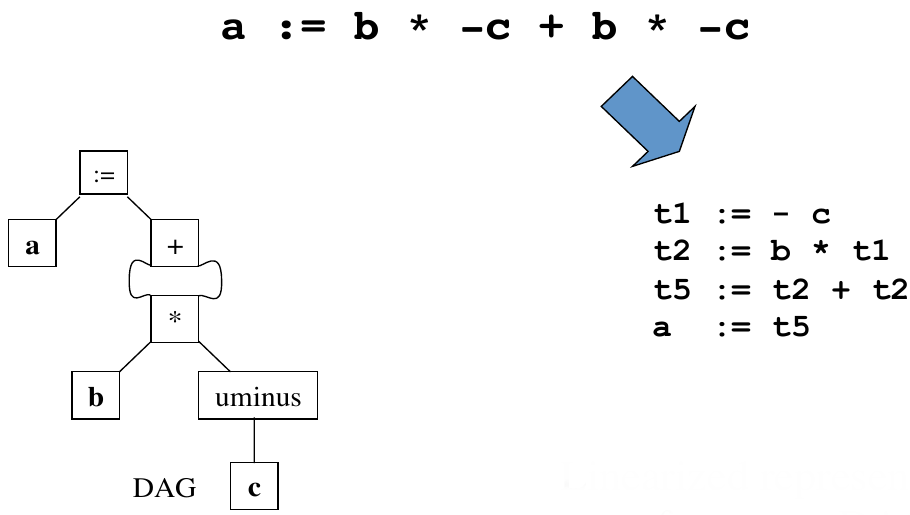
\includegraphics[scale=0.35]{res/image/tac_dag_rappresentation}
  \caption{Codice intermedio con \textit{Three-Address Code} dal DAG}
  \label{img:tag_dag_rappresentation}
\end{figure}

\subsection{Implementazione del Three-Address}
Il \textit{Three-Address Code} in memoria viene rappresentato mediante una
tabella dove vengono trascritti:
\begin{itemize}
\item ordine esecuzione istruzioni
\item operazioni
\item argomenti
\item variabile risultato
\end{itemize}

La differenza delle varie tecniche di rappresentazione mediante tabella \`e il
livello d'inferenza sulla variabile risultato (\textit{Triples}) e l'ordine
d'esecuzione delle istruzioni (\textit{Indirect Triples}),

\subsubsection{Quads}
Nella tabella delle \textbf{quadruple}(\textit{quads}) vengono archiviate tutte
le informazioni in modo esplicito.

\paragraph{pro}
Facile riarrangiare codice per ottimizzazioni globali.
\paragraph{cons}
Tanti temporanei.

\begin{figure}[H]
  \centering
  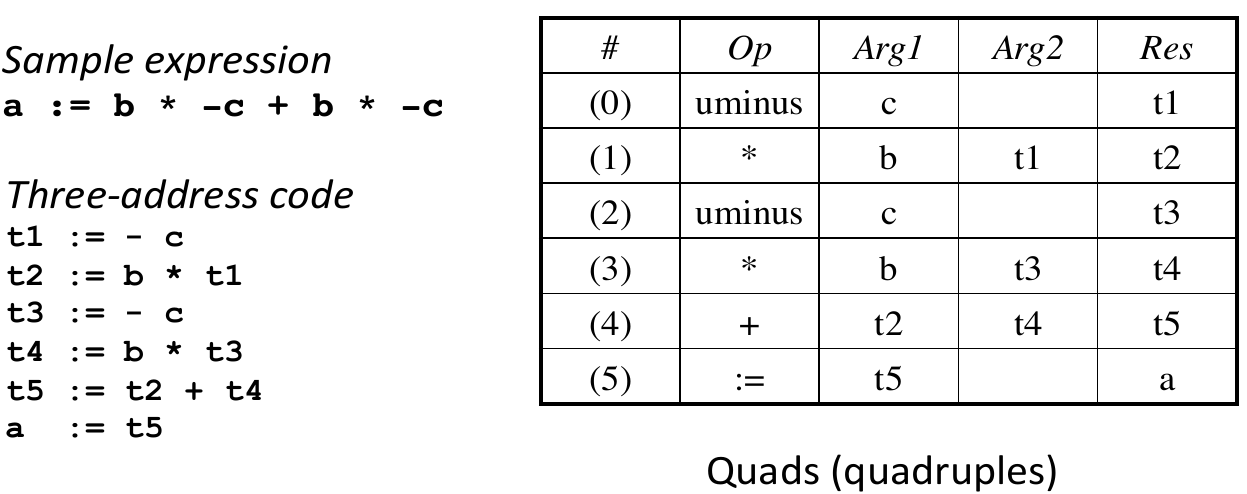
\includegraphics[scale=0.4]{res/image/quads}
  \caption{Quads}
  \label{img:quads}
\end{figure}

\subsubsection{Triples}
\label{sec:triples}
Nella tabella vengono salvate solo operazioni/operandi e l'ordine nella quale
eseguirle. Con la rimozione della colonna del risultato, la dichiarazione
delle temporanee diviene implicita e nelle operazioni dove prima erano presenti
si inserisce il numero dell'operazione da cui proviene il risultato.

\paragraph{pro}
Le temporanee sono impliciti (risparmio memoria).
\paragraph{cons}
Difficolt\`a nell'arrangiare il codice. Immagino sia per la necessit\`a di
dover aggiornare tutte le dipendenze con la nuova posizione del risultato.

\begin{figure}[H]
  \centering
  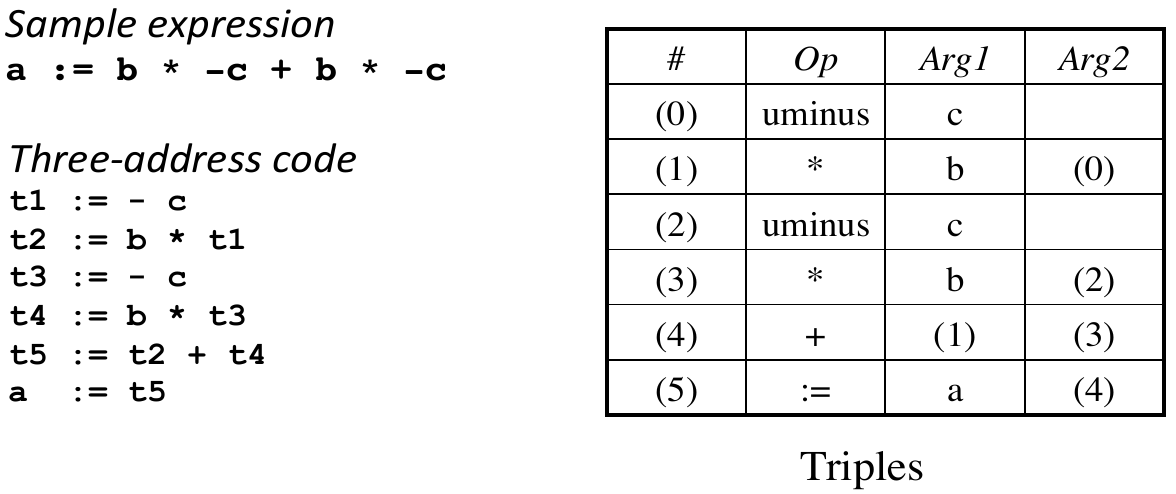
\includegraphics[scale=0.4]{res/image/triples}
  \caption{Triples}
  \label{img:triples}
\end{figure}

\subsubsection{Indirect Triples}
Un modo per ottere il meglio dei due mondi: facilit\`a di ordinamento del
codice (\textit{Quads}) e variabili temporanee implicite (\textit{Triples}),
si utilizzano le triple indirette. Semplicemente, si vanno ad utilizzare due
tabelle: una \`e la classica tripla (temporanee implicite) mentre la nuova
contiene l'ordine d'esecuzione delle operazioni da compiere. In questo modo il
riordinamento avverr\`a solo nella tabella con l'ordine del programma,
mantenendo invariati gli indici nella tripla. Da questa aggiunta si \`e
riusciti ad ottenere sia le temporanee implicite sia la facilita di ordinamento
del codice.

\begin{figure}[H]
  \centering
  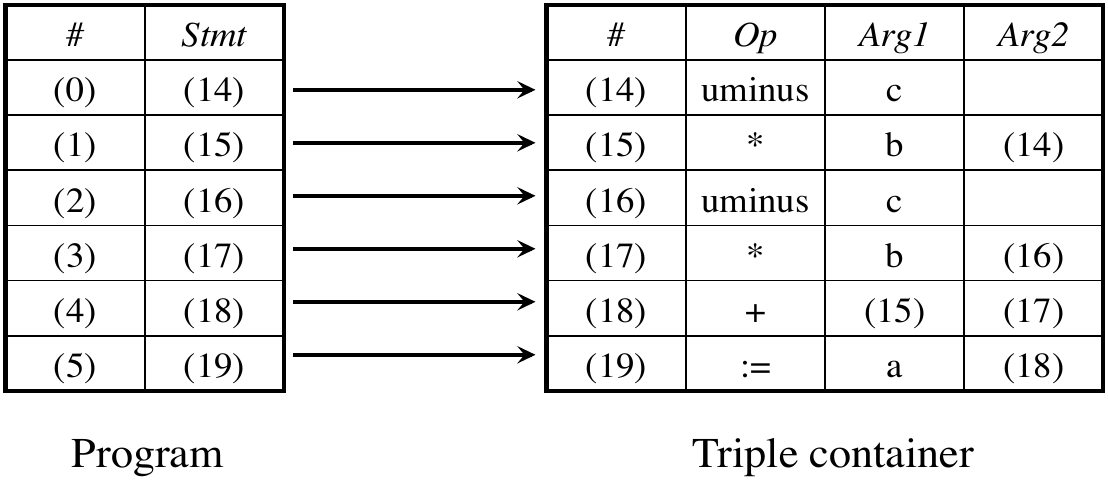
\includegraphics[scale=0.4]{res/image/indirect_triples}
  \caption{Indirect Triples}
  \label{img:indirect_triples}
\end{figure}

\subsection{Syntax-Directed Translation nel Three-Address Code}
La creazione del \textit{Three-Address Code} pu\`o avvenire immediatamente
utilizzando le \textit{Syntex Directed Translation}, specificando direttamente
nelle regole semantiche cosa produrre.

\begin{figure}[H]
  \centering
  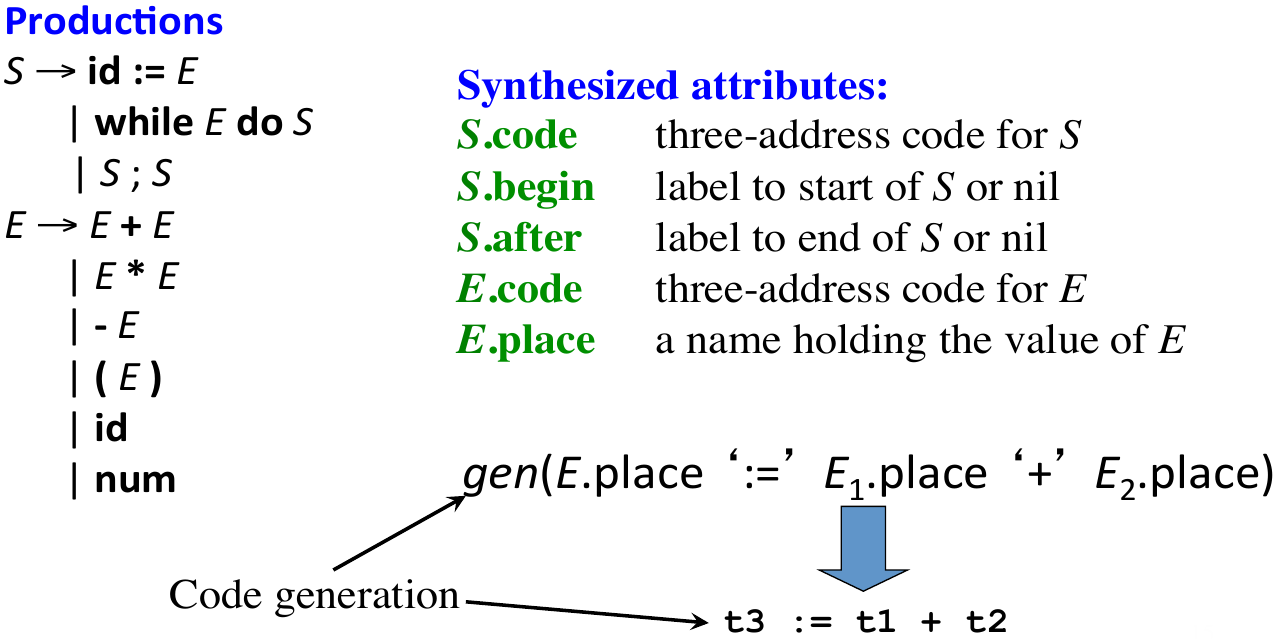
\includegraphics[scale=0.3]{res/image/traslation_tac}
  \caption{\textit{Three-Address Code} nel SDT}
  \label{img:traslation_tac}
\end{figure}

\subsection{Traduzione espressione logiche e relazionali}
Espressione booleane sono intese per rappresentare valori:
\begin{figure}[H]
  \centering
  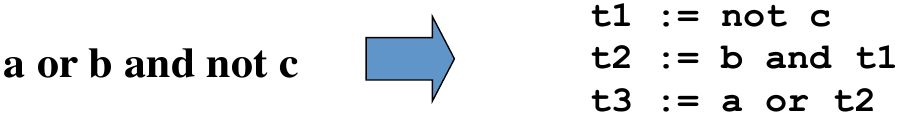
\includegraphics[scale=0.4]{res/image/bool_value}
  \caption{Operazioni booleane ritornano valori}
  \label{img:bool_value}
\end{figure}

Inoltre, vengono usate per alterare il flusso di controllo del programma:
\begin{figure}[H]
  \centering
  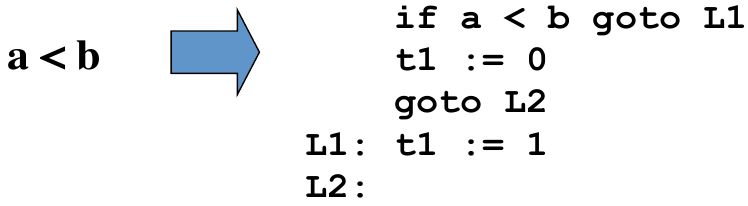
\includegraphics[scale=0.4]{res/image/bool_flow}
  \caption{Operazioni booleane sul controllo di flusso}
  \label{img:bool_flow}
\end{figure}

\subsection{Short-Circuit Code}
Gli operatori booleani $\&\&, \ ||, !$ sono tradotte in \textbf{salti}.

\begin{figure}[H]
  \centering
  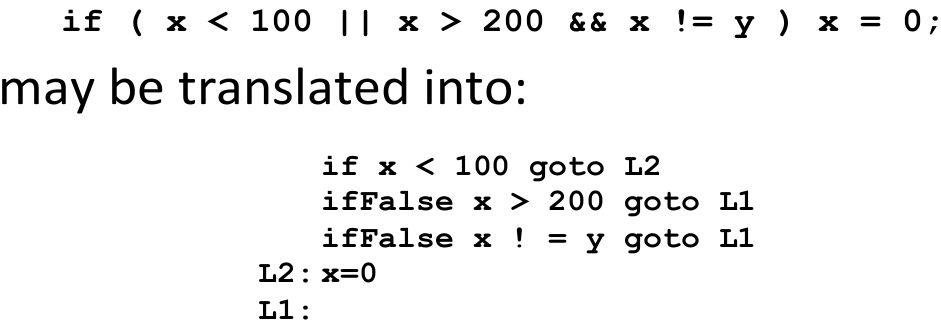
\includegraphics[scale=0.4]{res/image/short_circuit}
  \caption{Traduzione dei \textit{Short-Circuit Code}}
  \label{img:short_circuit}
\end{figure}

\subsection{Traduzione dei comandi flusso di controllo}
Il flusso di controllo \`e rilegato all'uso di salti per implementare i vari
branch decisionali in base alla guardia imposta. La completa traduzione sfrutta
tre attributi per poter descrivere i branch decisionali:
\begin{itemize}
\item $B.true$ - etichetta del ramo quando la guarda $B$ \`e vera
\item $B.false$ - etichetta del ramo quando la guarda $B$ \`e falsa
\item $S.next$ - etichetta dell'istruzione successiva ai corpi dei due rami
\end{itemize}

La regola semantica che produce la guarda conosce solo le etichette di dove
saranno eseguiti i salti ma la posizione delle etichette (ovvero la relativa
prima istruzione) sono conosciute dalla regola che effettivamente realizza i
corpi dei rami. Attraverso i tre attributi \textit{inherited} sopra citati si
potr\`a propagare i nomi delle etichette configurare nel nodo padre (la regola
della guarda) ai nodi figli (le regole dei corpi).

\begin{figure}[H]
  \centering
  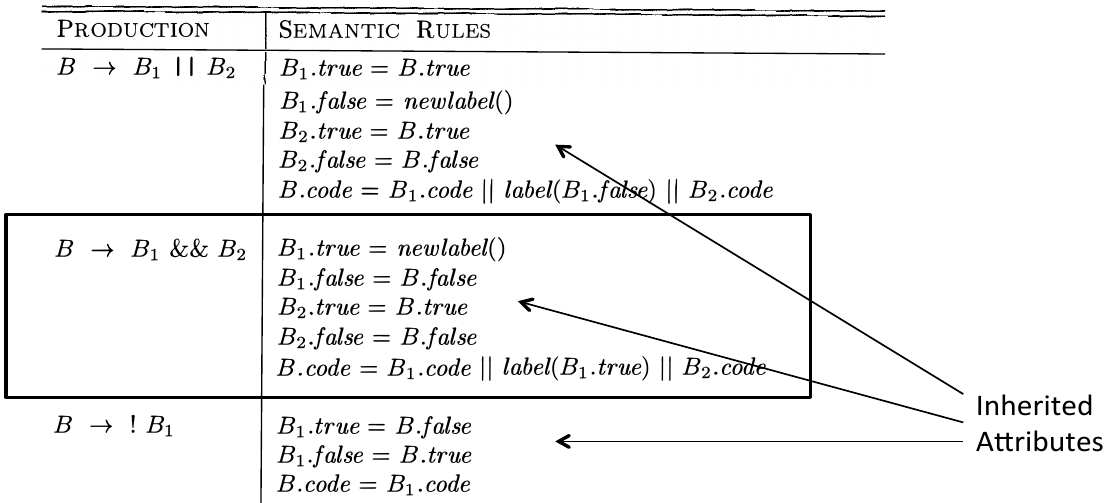
\includegraphics[scale=0.5]{res/image/propagation_label}
  \caption{Uso di attributi \textit{inherited} per propagare l'etichetta}
  \label{img:propagation_label}
\end{figure}

\subsection{Backpatching}
Il \textit{backpacthing} \`e una tecnica in cui esce dalla semantica del
programma e sfrutta il \textit{Translation Scheme} per evitare l'uso degli
attributi \textit{inherited} e sostituendoli con azioni di \textit{side-effect}
per inizializzare le etichette in modo corretto.

I \textit{side-effect} sono introdotti attraverso la chiamate a funzione
inserite nelle regole semantiche ed implementate attraverso un linguaggio di
programmazione. Questo trucco \`e possibile grazie alla libert\`a delle
\textit{translation schemes} in cui si va oltre alla semplice semantica della
grammatica.

L'idea del \textit{bankpatching} \`e produrre tutto il
\textit{three-address code} comprese le guardie ma non trascrivere le etichette
dei vari branch condizionali, il quale saranno calcolate in un secondo tempo.
Nel parsing della grammatica si riscontrano due momenti decisivi:
\paragraph{Guardia}
All'incontro della guarda si richiedono i propri indirizzi di memoria nel
quale verranno salvate in due list: \textit{.truelist} e \textit{.falselist}.
Nella \textit{.truelist} si inserisce l'indirizzo della stessa guardia e nella
\textit{.falselist} l'indirizzo dell'istruzione immediatamente successiva
(il salto al corpo del branch quando la guardia \`e falsa). Infine si stampano
i controlli di flusso lasciando dei segnaposti sulle label.

\begin{figure}[H]
  \centering
  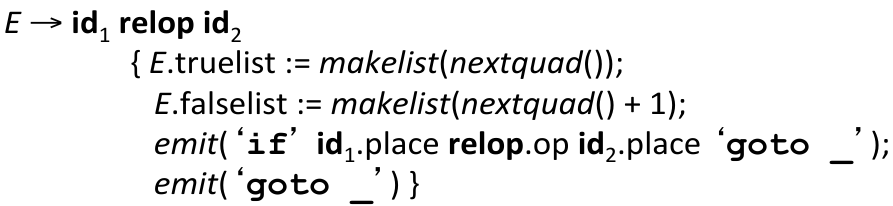
\includegraphics[scale=0.5]{res/image/condition_backpatching}
  \caption{\textit{Semantic Rules} per la guardia}
  \label{img:condition_backpatching}
\end{figure}

Attraverso comandi \textit{makelist} e \textit{nextquad} si va a uscire dalla
semplice denotazione semantica ma ad avviare proprie procedure per garantire
la rimozione degli attributi ereditati:
\begin{itemize}
\item \textit{makelist} costruisce la lista in cui verranno messi tutti i
\textit{three-address code} relativi alle istruzioni di salto con i segnaposto
usati per rappresentare l'indirizzo di destinazione, e ritorna il puntato ad
essa.
\item \textit{nextquad} ritorna l'indirizzo di memoria occupato dall'istruzione
corrente. Nota: \textit{nextquad} \`e un indirizzo di memoria a tutti gli
effetti ed \`e quindi possibile utilizzare l'aritmetica dei puntatori.
\end{itemize}

\paragraph{Blocchi condizionali}
Nelle produzioni della grammatica si pu\'o beneficiare di una vista ad alto
livello della sintassi, in questo caso dei blocchi che compongono il programma.
Nella produzione si modella l'inizio e la fine dei blocchi e questo permette di
agire per sapere quando eseguire le operazioni di \textit{backpatching}.

La grammatica viene aumentata con l'inserimento di un
\textit{marker nonterminal} esattamente nel punto in cui il blocco finisce e
comincia quello successivo. Al suo sviluppo verr\'a richiesto la posizione di
memoria della prima istruzione del blocco in cui risiede che \`e esattamente
l'indirizzo di memoria della prima istruzione del blocco successivo.

Ora, a seconda dell'operazione, il \textit{backpatching} agir\'a su una delle
due liste: (\textit{.truelist} e \textit{.falselist}), sostituendo i segnaposto
con l'indirizzo acquisito nello sviluppo del \textit{marker}.

\begin{figure}[H]
  \centering
  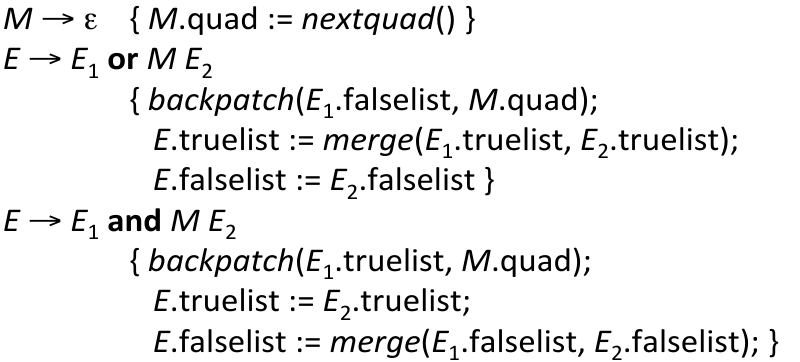
\includegraphics[scale=0.5]{res/image/block_backpatching}
  \caption{\textit{Semantic Rules} per i blocchi}
  \label{img:block_backpatching}
\end{figure}
